% Chapter 1
\setchapterimage{jet}
\setchapterpreamble[u]{\margintoc}
\chapter{Fusion: general introduction} % Main chapter title
\label{Chapter1} % For referencing the chapter elsewhere, use \ref{Chapter1} 
\section{Thermonuclear fusion: principles}
\lipsum[6]
\lipsum[6]

\begin{figure} [h]
    \centering
    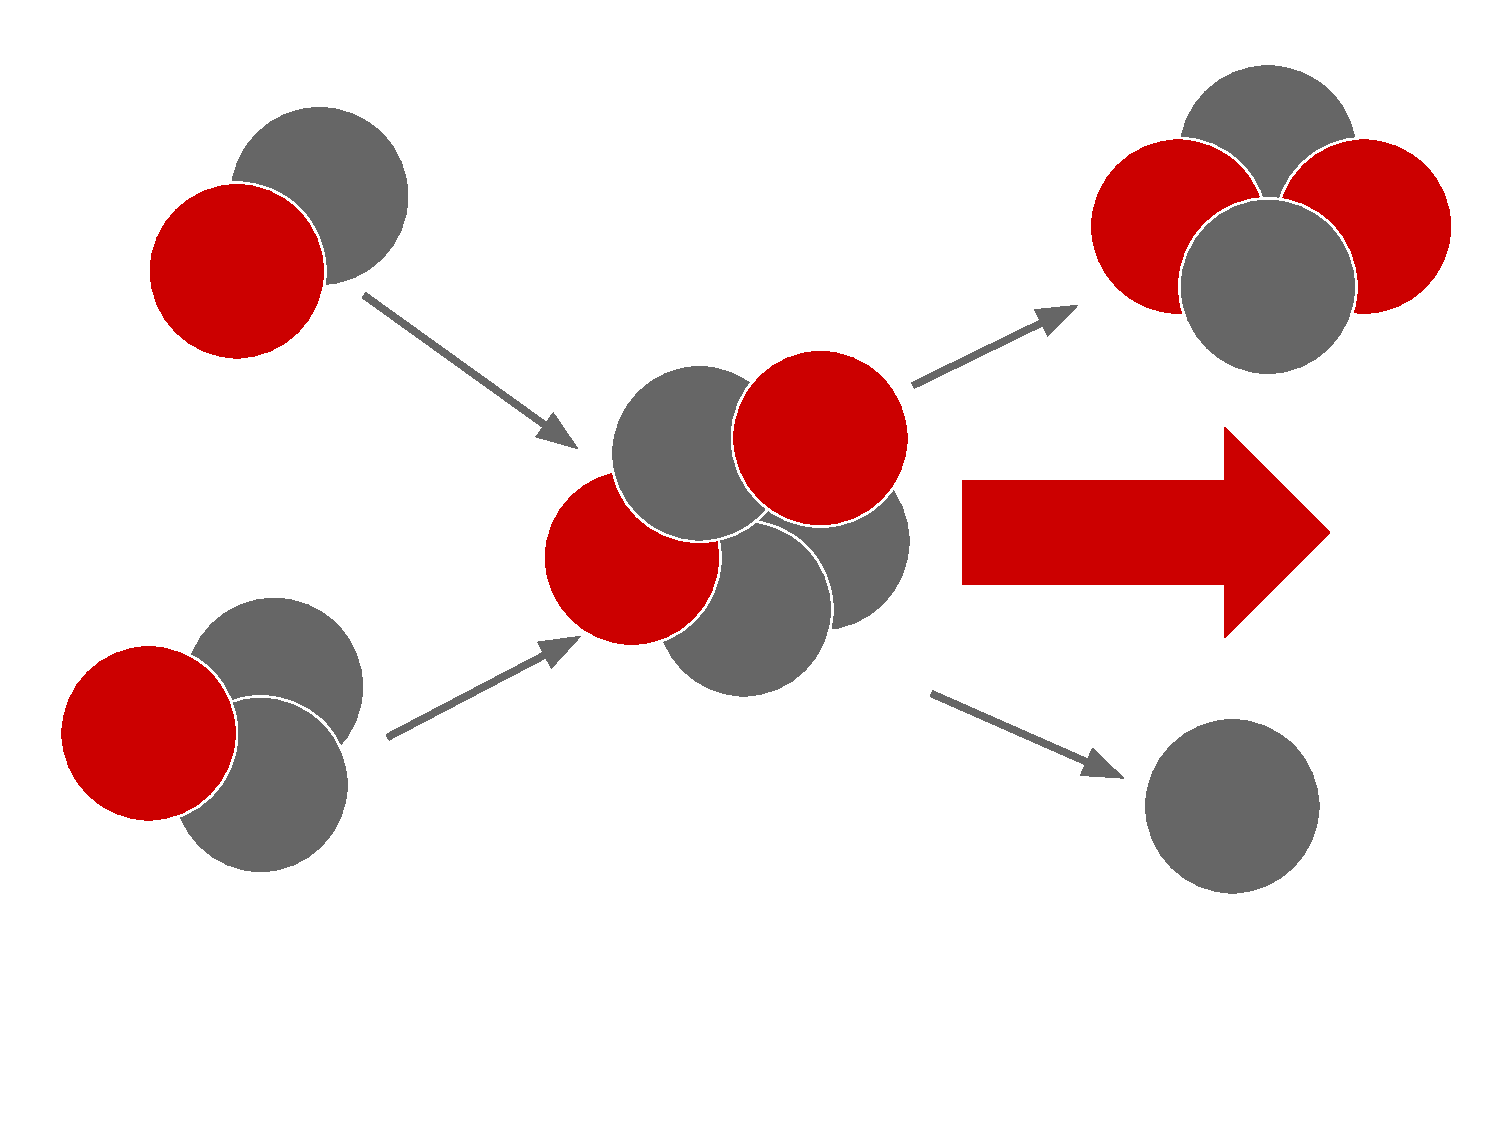
\includegraphics[width=\linewidth]{Figures/Chapter1/nuc_fus.pdf}
    \caption{My caption}
\end{figure}

\lipsum[6]
\lipsum[6]

\begin{figure} [h]
    \centering
    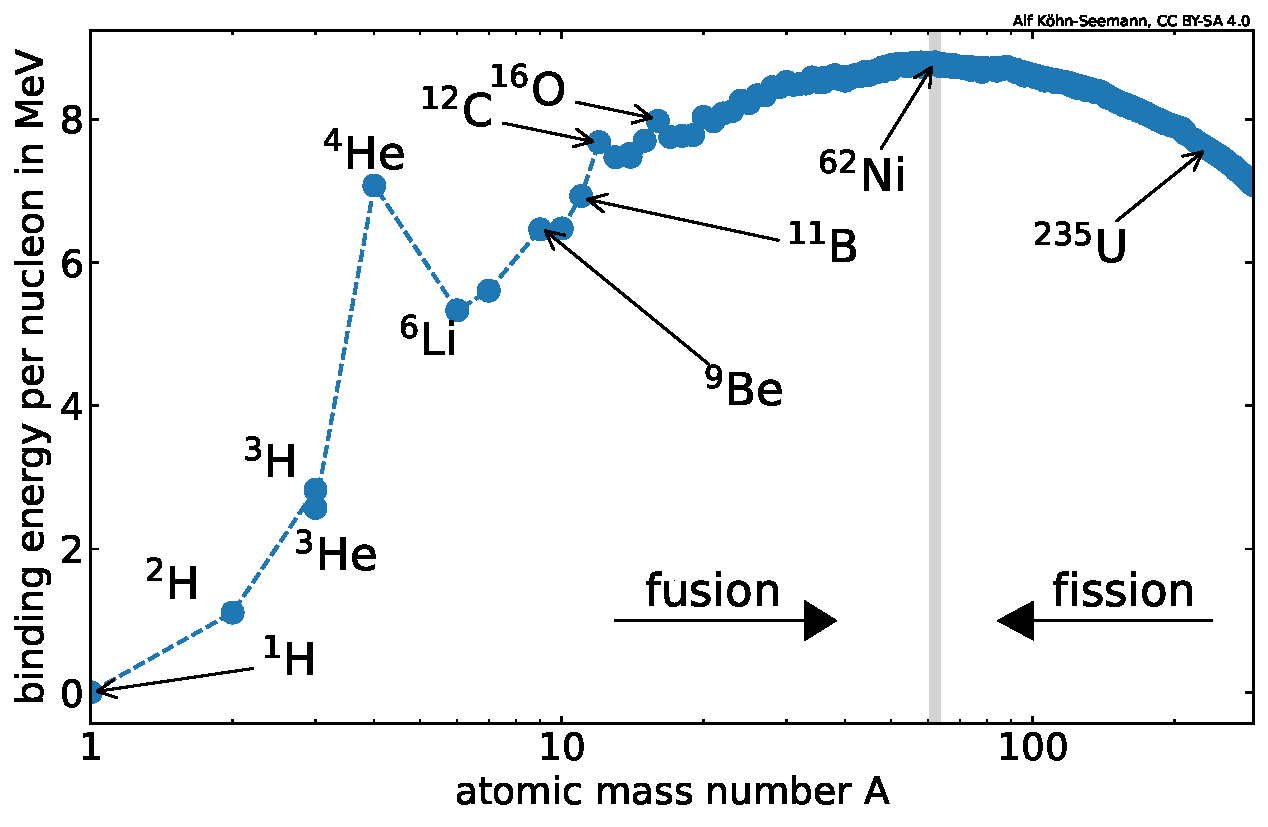
\includegraphics[width=\linewidth]{Figures/Chapter1/binding_energy_per_nucleon.pdf}
    \caption{My caption}
\end{figure}

\lipsum[6]
\lipsum[6]

\begin{figure} [h]
    \centering
    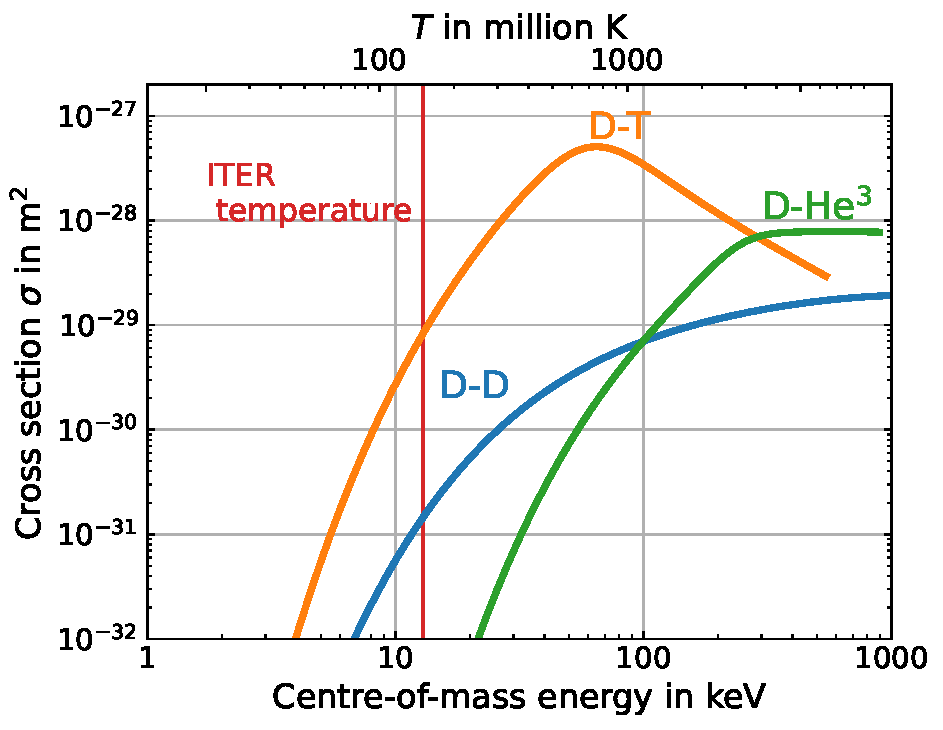
\includegraphics[width=\linewidth]{Figures/Chapter1/cross_sections_vs_temperature__Bosch.pdf}
    \caption{My caption}
\end{figure}


\subsection{Tokamaks: how to put the sun in a bottle}

\lipsum[6]
\lipsum[6]

\begin{figure}
    \centering
    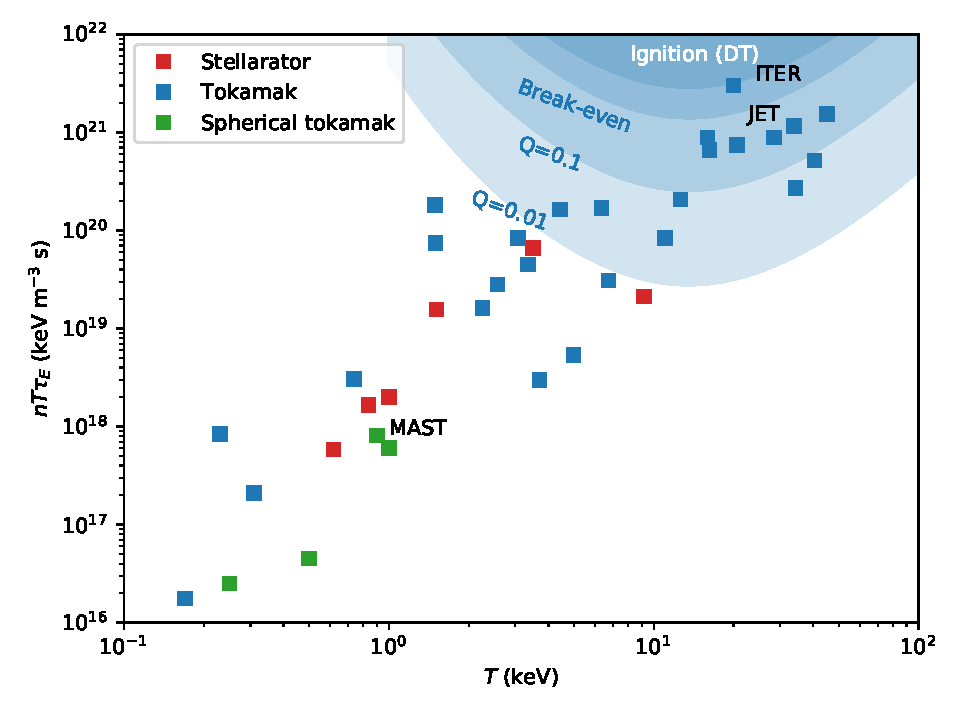
\includegraphics[width=\linewidth]{Figures/Chapter1/triple_product_vs_T.pdf}
    \caption{My caption}
\end{figure}

\subsection{Main challenges}
\section{Plasma-surface interactions in tokamaks}
\lipsum[6]
\lipsum[6]

\subsection{H/W, He/W and He/H interactions}
\subsection{Experimental methods}
\subsection{Modelling methods}
\section{Roadmap}



